% Unterstützung für Links und PDF Metadaten
\documentclass[
  bibliography=totoc,     % Literatur im Inhaltsverzeichnis
  captions=tableheading,  % Tabellenüberschriften
  titlepage=firstiscover, % Titelseite ist Deckblatt
]{scrartcl}

% Paket float verbessern
\usepackage{scrhack}

% Warnung, falls nochmal kompiliert werden muss
\usepackage[aux]{rerunfilecheck}

% unverzichtbare Mathe-Befehle
\usepackage{amsmath}
% viele Mathe-Symbole
\usepackage{amssymb}
% Erweiterungen für amsmath
\usepackage{mathtools}

% Fonteinstellungen
\usepackage{fontspec}
% Latin Modern Fonts werden automatisch geladen
% Alternativ zum Beispiel:
%\setromanfont{Libertinus Serif}
%\setsansfont{Libertinus Sans}
%\setmonofont{Libertinus Mono}

% Wenn man andere Schriftarten gesetzt hat,
% sollte man das Seiten-Layout neu berechnen lassen
\recalctypearea{}

% deutsche Spracheinstellungen
\usepackage{polyglossia}
\setmainlanguage{german}


\usepackage[
  math-style=ISO,    % ┐
  bold-style=ISO,    % │
  sans-style=italic, % │ ISO-Standard folgen
  nabla=upright,     % │
  partial=upright,   % ┘
  warnings-off={           % ┐
    mathtools-colon,       % │ unnötige Warnungen ausschalten
    mathtools-overbracket, % │
  },                       % ┘
]{unicode-math}

% traditionelle Fonts für Mathematik
\setmathfont{Latin Modern Math}
% Alternativ zum Beispiel:
%\setmathfont{Libertinus Math}

\setmathfont{XITS Math}[range={scr, bfscr}]
\setmathfont{XITS Math}[range={cal, bfcal}, StylisticSet=1]

% Zahlen und Einheiten
\usepackage[
  locale=DE,                   % deutsche Einstellungen
  separate-uncertainty=true,   % immer Fehler mit \pm
  per-mode=symbol-or-fraction, % / in inline math, fraction in display math
]{siunitx}

% chemische Formeln
\usepackage[
  version=4,
  math-greek=default, % ┐ mit unicode-math zusammenarbeiten
  text-greek=default, % ┘
]{mhchem}

% richtige Anführungszeichen
\usepackage[autostyle]{csquotes}

% schöne Brüche im Text
\usepackage{xfrac}

% Standardplatzierung für Floats einstellen
\usepackage{float}
\floatplacement{figure}{htbp}
\floatplacement{table}{htbp}

% Floats innerhalb einer Section halten
\usepackage[
  section, % Floats innerhalb der Section halten
  below,   % unterhalb der Section aber auf der selben Seite ist ok
]{placeins}

% Seite drehen für breite Tabellen: landscape Umgebung
\usepackage{pdflscape}

% Captions schöner machen.
\usepackage[
  labelfont=bf,        % Tabelle x: Abbildung y: ist jetzt fett
  font=small,          % Schrift etwas kleiner als Dokument
  width=0.9\textwidth, % maximale Breite einer Caption schmaler
]{caption}
% subfigure, subtable, subref
\usepackage{subcaption}

% Grafiken können eingebunden werden
\usepackage{graphicx}
% größere Variation von Dateinamen möglich
\usepackage{grffile}

% schöne Tabellen
\usepackage{booktabs}

% Verbesserungen am Schriftbild
\usepackage{microtype}

% Literaturverzeichnis
\usepackage[
  backend=biber,style=numeric,sorting=none
]{biblatex}
% Quellendatenbank
\addbibresource{lit.bib}
\addbibresource{programme.bib}

% Hyperlinks im Dokument
\usepackage[
  unicode,        % Unicode in PDF-Attributen erlauben
  pdfusetitle,    % Titel, Autoren und Datum als PDF-Attribute
  pdfcreator={},  % ┐ PDF-Attribute säubern
  pdfproducer={}, % ┘
]{hyperref}
% erweiterte Bookmarks im PDF
\usepackage{bookmark}

% Trennung von Wörtern mit Strichen
\usepackage[shortcuts]{extdash}

\usepackage{tikz}
\usepackage{tikzscale}
\usetikzlibrary{arrows.meta}

\author{%
  Thomas Honermann\\%
  \href{mailto:thomas.honermann@tu-dortmund.de}{thomas.honermann@tu-dortmund.de}%
  \texorpdfstring{\and}{,}%
  Yascha Franz\\%
  \href{mailto:yascha.franz@tu-dortmund.de}{yascha.franz@tu-dortmund.de}%
}
\publishers{TU Dortmund – Fakultät Physik}

% Einstellungen hier, z.B. Fonts



\begin{document}
% Text hier
\titlehead{
\includegraphics[height=1.5cm]{ressources/logo.jpg}}
\title{Protokoll zum Versuch  \\ }
\date{Durchführung:  \\ Abgabe:  }

% 7 \, s vor Korrekturabgabe:

\maketitle
\tableofcontents
\newpage

\section{Zielsetzung und Theorie}

% \subsection{Zielsetzung}
Aus der Medizin bekannt und in vielen Bereichen der Physik und anderen
Naturwissenschaften ist das zerstörungsfreie Messverfahren der Kernspinresonanz.
Ortsabhängige Vorgänge lassen sich mithilfe des Phänomens der Kernspinresonanz
unter Beobachtung magnetischer Gradientenfelder bildgebend darstellen. \\
In diesem Versuch sollen dazu die Spin-Gitter-Relaxation und die
Spin-Spin-Relaxation genauer betrachtet werden. Explizit betrachtet werden
sollen dazu die charakteristischen Relaxationszeiten und die zugehörigen
Diffusionskoeffizienten von Wasser. Dazu wird die magnetische Resonanz an
Protonen genutzt.  


\subsection{Theorie}
\noindent Die \enquote{nuclear magnetic resonance}, kurz NMR, beschreibt Phänomene, welche
bei der Wechselwirkung zwischen elektromagnetischer Strahlung und Materie in
Erscheinung treten. Die Energieniveaus, welche sich für verschiedene magnetische
Felder der Flussdichte $B$ ergeben, stehen dabei in direkter Verbindung zu den
Orientierungen der magnetischen Momente der Atome im angelegten magnetischen
Feld \cite{nmr_relaxation}.
\subsection{Kern- und Elektronenmagnetismus}
\noindent Magnetisch wechselwirkende Kerne besitzen neben einem magnetischen
Moment einen Drehimpuls $\vec{J}$. Dieser ist proportional zum magnetischen
Moment $\vec{\mu} = \gamma \cdot \vec{J}$, wobei der Proportionalitätsfaktor
$\gamma$ den gyromagnetischen Faktor beschreibt. Unter Einfluss eines äußeren
magnetischen Feldes mit einer Flussdichte $B$ koppeln das magnetische Moment und das magnetische Feld
zu einem Drehmoment $\vec{D} = \vec{\mu} \times B = \frac{d \vec{J}}{dt}$.
Für konstante, homogene Felder mit fester räumlicher Orientierung
(beispielsweise in z-Richtung) präzediert das magnetische Moment $\vec{\mu}$
in Richtung des magnetischen Feldes. Die zur Präzession gehörige
Frequenz ist dabei die Lamorfrequenz $\nu = \frac{\omega}{2 \cdot \pi} =
\frac{\gamma \cdot B_z}{2 \cdot \pi}$. Der Index $z$ der magnetischen Feldstärke
gibt dabei an, in welche Richtung (hier z-Richtung) das Feld
ausgerichtet ist. Die Frequenz $\omega$ entspricht der zur Lamorfrequenz gehörigen
Winkelgeschwindigkeit.
\subsection{Magnetisierung und Relaxation}
\noindent Um Effekte der Kernspinresonanz untersuchen zu können, ist ein
statisches Magnetfeld $B_\text{stat.}$ notwendig. Zusätzlich befindet sich die Probe in
einer Spule, in welche durch weitere, kurze Strompulse magnetische Felder $B_\text{puls.}$ induziert
werden, welche unabhängig vom statischen Feld sind. Die Pulse lassen sich dazu nutzen, das thermische Gleichgewicht der
Probe zu stören und die Magnetisierung um einen Winkel proportional zur
Pulsdauer zu drehen. \\
\noindent Nach Abklingen des kurzen Strompulses und Verschwinden des
Magnetfeldes $B_\text{puls.}$ beginnt die angeregte Magnetisierung der Probe ins thermische
Gleichgewicht zurück zu relaxieren. Das Relaxiationsverhalten wird dabei durch
die Bloch-Gleichungen
\begin{align*}
  \left(\frac{dM_x}{dt} \right) &= \left(-\frac{M_x}{T_2} \right),  \\
  \left(\frac{dM_y}{dt} \right) &= \left(-\frac{M_y}{T_2} \right) 
\end{align*}
\begin{align}
  \left(\frac{dM_z}{dt} \right) &= \left(\frac{M_0 - M_z}{T_1} \right)
  % M_z = M_0 \cdot \left(1 - \exp{\left(-\frac{t}{T_1}\right)}\right)
  \label{eqn:01}
\end{align}
\noindent beschrieben. Der Index $i$ gibt auch hier wieder die Richtung der
Magnetisierung an, $M_0$ beschreibt die Magnetisierung im thermischen
Gleichgewicht, $T_1$ beschreibt die Spin-Gitter-Relaxationszeit und $T_2$
entspricht der Spin-Spin-Relaxationszeit. \\
\subsubsection{Spin-Gitter-Relaxationszeit}
Die Relaxationszeit in z-Richtung wird in den Bloch Gleichungen 1 bis 2
durch $T_1$ beschrieben. Diese Zeitkonstante beschreibt dabei die Eigenschaften
des Spinsystems sowie die Eigenschaften dessen unmittelbarer Umgebung. Für große
Werte von $T_1$ besteht lediglich eine schwache Kopplung von Spinsystem und
Umgebung, kleine Werte lassen auf eine starke Kopplung beider Systeme schließen.
Während der Relaxation wird die potentielle Energie der Kernspins der Probe in
eine Gitterschwingung umgewandelt. \\
\subsubsection{Spin-Spin-Relaxation}
\noindent Während Spin-Spin-Relaxation auf die z-Richtung beschränkt ist, findet
die Spin-Spin-Relaxation in der xy-Ebene statt. In dieser Ebene resultiert die
Magnetisierung aus allen Präzessionsbewegungen um die z-Achse. Da die Magnetisierung nicht
volkommen homogen über die Ebene verteilt ist, unterscheiden sich die zu den
Präzessionen gehörigen Lamor-Frequenzen gering voneinander, sodass die
Spins bereits nach kurzer Zeit nicht weiter in Phase schwingen \cite{nmr}.
Explizit äußert sich die Dephasierung dabei auf zwei verschiedenen Arten. Zum
einen sorgt die inhomogene Verteilung für eine statische Feldinhomogenität, deren
Reversibilität im Hahn-Echo-Verfahren genutzt wird, um die Feldinhomogenität zu
minimieren und $T_2$ bestimmen zu können. Zum anderen zeigt sich eine irreversible
Dekohärenz, angeregt beispielsweise durch Stoßprozesse oder eine $T_1$-Relaxation,
welche Einfluss auf den $T_2$-Parameter nimmt.
\subsection{Diffusion}
\noindent Für sphärische Moleküle mit dem Radius $r$ liefert die
Einstein-Stokes Gleichung
\begin{align}
  D = \frac{k_B \cdot T}{6 \cdot \pi \cdot \eta \cdot r}
  \label{eqn:02}
\end{align}
\noindent eine Möglichkeit, aus der Diffusionskonstanten $D$ den Molekülradius
$r$ zu bestimmen. Dieser ist Abhängig von der Temperatur $T$ der Moleküle sowie
der Viskosität $\eta$. Die Boltzmann-Konstante $k_B$ drückt ebenso wie der
Faktor $\pi$ lediglich eine Proportionalität aus \cite{stokes}. \\
\noindent In einem magnetischen Gradientenfeld führt die Verschiebung der Spins
aufgrund der Diffusionsprozesse während der $T_2$ Relaxation zu einer
zusätzlichen Signalabnahme. Mit der Diffusions-Zeitkonstante
\begin{align}
  T_D = \frac{3}{\gamma^2 \cdot \tau^2 \cdot G^2 \cdot D}
  \label{diffusion_constant}
\end{align}
lässt sich schließlich
der Diffusionskoeffizient der Einstein-Stokes Gleichung \ref{eqn:02} bestimmen,
welcher sich in einen Molekülradius $r$ umrechnen lässt. Der Faktor $\gamma$
beschreibt dabei noch immer das gyromagnetische Verhältnis, $\tau$ entspricht
dem zeitlichen Abstand der Pulse und $G$ stellt den magnetischen Feldgradienten
dar
% , welcher sich aus $G = 2 \cdot \pi \cdot d_f \cdot(\gamma \cdot d)^{-1}$
% berechnen lässt. Der Durchmesser des gemessenen Spektrums $d_f$ ist dabei in
% $\si{\hertz}$ angegeben, $d$ bezeichnet den Innendurchmesser der Probe
\cite{sample}.
\noindent Unter dem \enquote{freien Induktionsfall} (FID) ist die Relaxation
der Magnetisierung zurück ins thermische Gleichgewicht bekannt, nachdem ein
A-Puls für eine Verkippung innerhalb der xy-Ebene gesorgt hat. Das
Relaxationsverhalten lässt sich dabei beschreiben durch die Gleichungen
\begin{align}
  M_x(t) &= M_0 \cdot \cos{(\omega_0 t)} \cdot \exp{\left( - \frac{t}{T_2}\right)} \qquad \text{und} \\
  M_y(t) &= - M_0 \cdot \sin{(\omega_0 t)} \cdot \exp{\left( - \frac{t}{T_2}\right)}.
\end{align}
\noindent Das sich periodisch ändernde Magnetfeld bewirkt dadurch nach den
Lenz'schen Regeln einen Induktionsstrom.


\section{Aufbau und Durchführung}

% \subsection{Aufbau}
% \noindent Im Wesentlichen besteht der Versuchsaufbau aus einem Szintillatortank
mit einem Volumen $V = \SI{50}{\liter}$ und zwei angeflanschten PMTs, sowie
einem Rack mit verschiedenen elektrischen Bauteilen zur Signalverarbeitung. Zu
diesen Geräten gehören Verzögerungsleitungen (verschieden lange Kabelverbindungen
mit Verzögerunsgleistungen im Bereich einiger Nanosekunden), Diskriminatoren
zur Festlegung von Schwellspannungen, einem Doppelimpulsgenerator, einer
Koinzidenzschaltung, Impulszählgeräten, einem Monoflop, einem
Time-Amplitude-Converter (TAC) sowie einem Multi-Channel-Analyzer (MCA), dessen
Signale von einem PC ausgewertet werden. Zusätzlich steht ein Oszilloskop bereit.
Die Bauelemente sind alle in Abbildung \ref{fig:02} aufgeführt.  \\
\newline
\noindent Die Ausgängssignale der Photomultiplier sind über
Verzögerungsleitungen mit Diskriminatoren verbunden und werden anschließend an
eine Koinzidenzschaltung weitergeleitet. Diese ist ebenfalls mit einem
Doppelimpulsgenerator verbunden. Die Koinzidenzschaltung leitet lediglich im
Falle eines simultanen Signaleingangs der Signale zweier PMT ein Signal weiter,
zu Kalibrierungszwecken kann der Doppelimpulsgenerator das erforderliche zweite
Eingangssignal geben. \\
\noindent Am Anschluss an die Koinzidenzschaltung folgen zwei AND-Gitter, wovon
eines direkt, ein zweites erst nach einer weiteren Verzögerungsleitung und einem
Monoflip vom Signal erreicht wird. Der Monoflip dient dabei einer Eingrenzung
der Suchzeit, innerhalb welcher die Myonzerfälle zu erwarten sind. Die
Verzögerungsleitung soll eine Verzögerungszeit $\Delta t = \SI{30}{\nano\second}$
gewährleisten. Die beiden AND-Gitter, die ein Signal jeweils aus der
Koinzidenzschaltung direkt beziehen, erhalten ihr zweites Signal aus dem
Monoflop. Dieser erhält sein Signal um die Zeitspanne $\Delta t$ zeitversetzt.
Wird er getriggert, sperrt er für die Suchzeit $T_s$ das Startsignal am ersten
AND-Gitter und gibt es nach der Suchzeit wieder frei. Ein Signaleingang
innerhalb der Suchzeit hingegen schaltet ein Stopp-Signal. Die Start und
Stop-Signale werden jeweils einzeln gezählt, die Signalverarbeitung geschieht
über den TAC und den MCA am PC \cite{anleitung}.   


% \subsection{Aufbau und Durchführung}
\noindent Die Schaltungen werden entsprechend der Schaltskizzen \ref{fig:03} bis
\ref{fig:07} auf die Steckplatine wie in Abbildung \ref{aufbau} dargestellt
aufgesteckt. Zu beachten ist dabei, dass die Schaltungen erst mit Spannung
versorgt werden, wenn die Widerstände dem Operationsverstärker vorgeschaltet
sind, um Schäden am elektrischen Bauteil zu vermeiden. \\
\FloatBarrier
\begin{figure}
  \centering
  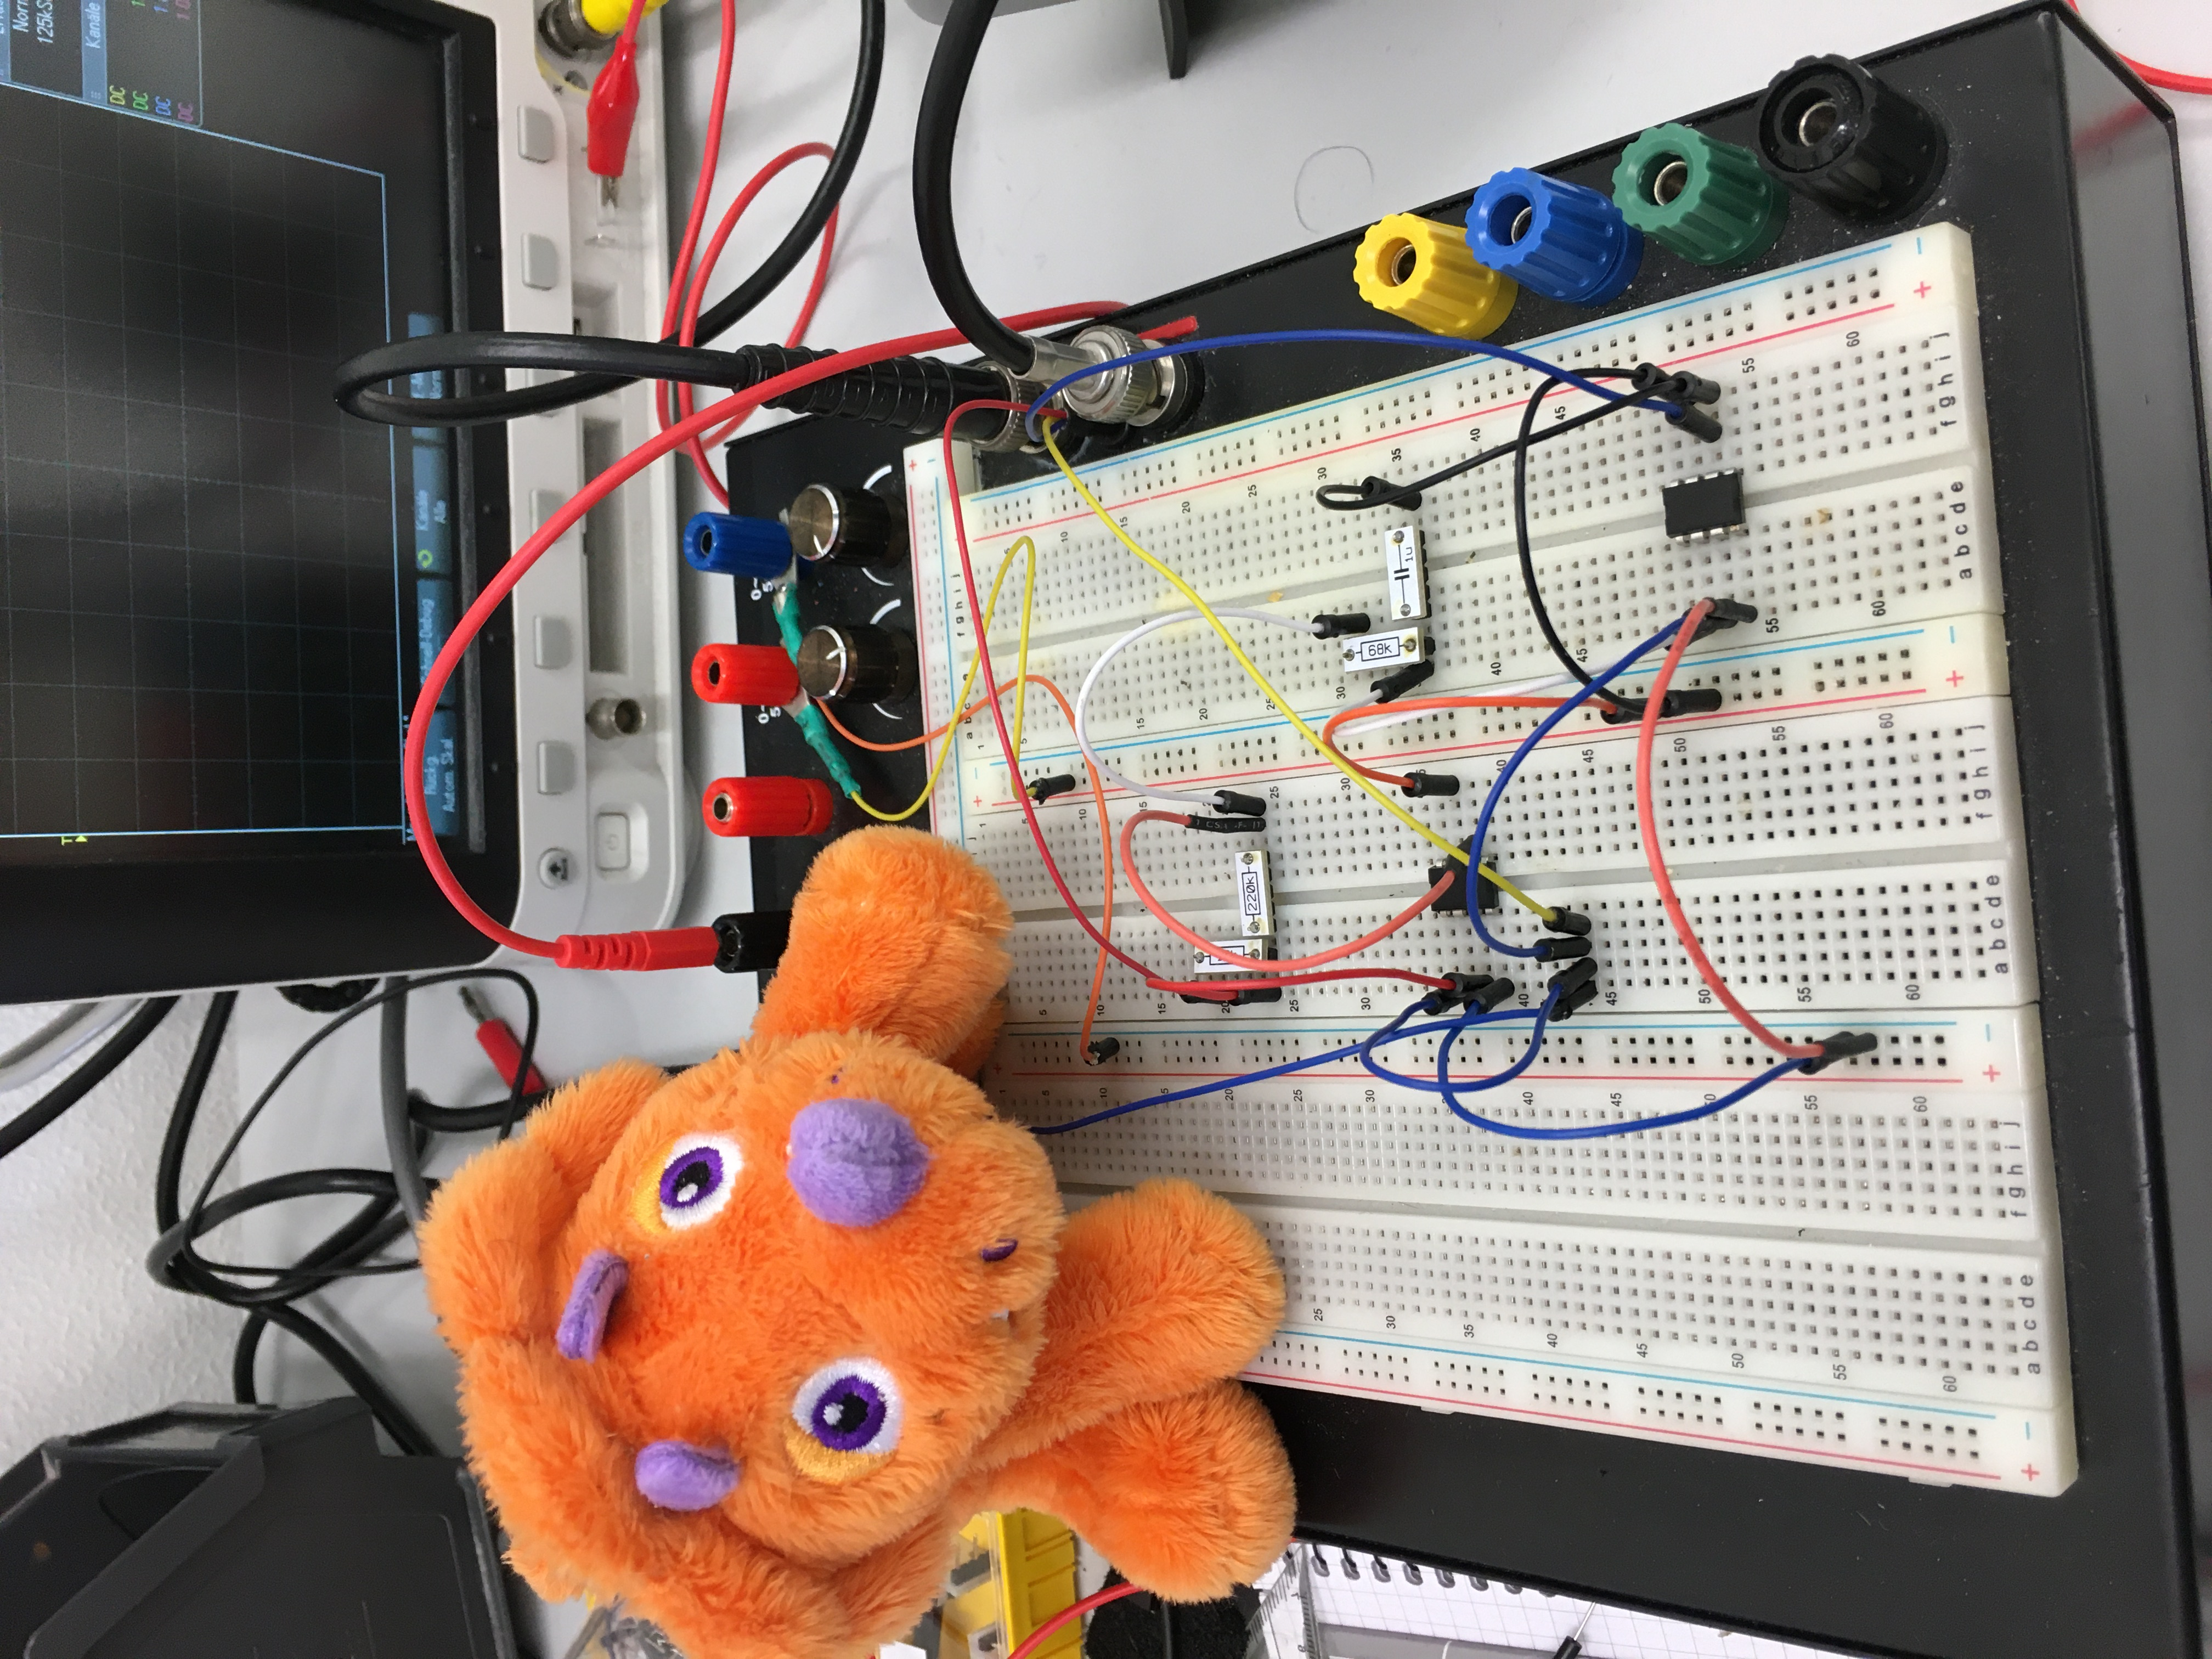
\includegraphics[scale=0.07]{ressources/aufbau.JPG}
  \caption{Versuchsaufbau zur Signalgeneratorschaltung.}
  \label{aufbau}
\end{figure}
\FloatBarrier
\noindent Für die Schaltung zum invertierenden Linearverstärker werden die
Widerstände $R_1 = \SI{1}{\kilo\ohm}$ und $R_2 = \SI{100}{\kilo\ohm}$
verwendet. Die Betriebsspannung des Operationsverstärkers vom Typ LM741
liegt im Spannungsbereich von $U_1 = -\SI{15}{\volt}$ bis $U_2 = \SI{15}{\volt}$
\cite{datenblatt}. Für die Messungen wird eine Eingangsspannung
$U_e = -\SI{50}{\milli\volt}$ angelegt. Die Frequenz wird über mehrere Dekaden
variiert, das Eingangssignal ist dabei sinusförmig. Dabei lässt sich  neben der Ausgangsspannung
die Phasenverschiebung zwischen Eingangs- und Ausgangssignal mit dem
Oszilloskop messen und die erwartete Abnahme für hohe Frequenzen untersuchen.
Zu beachten ist, dass das Verstärkungssignal während der
Durchführung unverzerrt ist. Die Messung wird für verschiedene Widerstände
zweimal wiederholt. \\
\noindent Der Umkehr-Integrator wird mit dem Widerstand $R = \SI{10}{\kilo\ohm}$
und einem Kondensator der Kapazität $C = \SI{100}{\nano\farad}$ realisiert.
Die gewählte Zeitkonstante ist dabei durch Untersuchung der Proportionalität
zwischen Ausgangsspannung und dem Kehrwert der Frequenz (sinusförmiges
Eingangssignal) zu prüfen. Gemessen werden bei dieser Schaltung die Eingangs-
und Ausgangsspannungen in Abhängigkeit von der Frequenz. \\
\noindent Analog zum Umkehr-Integrator wird die Messung des invertierenden
Differenzierers durchgeführt. Dazu wird der Widerstand durch einen Kondensator
der Kapazität $C = \SI{20}{\nano\farad}$ und der Kondensator der vorherigen
Schaltung durch einen Widerstand $R = \SI{100}{\kilo\ohm}$ ersetzt. \\
\noindent Im Anschluss daran wird eine nicht-invertierende
Schmitt-Trigger-Schaltung gemäß Abbildung \ref{fig:07} aufgebaut. Für die
Widerstände gilt $R_1 = \SI{10}{\kilo\ohm}$ und $R = \SI{100}{\kilo\ohm}$.
Zu beachten ist hierbei die Vertauschung des nicht-invertierenden Signaleingangs
mit dem invertierenden Signaleingang. In Millivolt-Schritten wird ausgehend vom
Startwert $U = \SI{0}{\volt}$ die Amplitude des sinusförmigen Eingangssignals
erhöht und mithilfe des Oszilloskops die Amplitude ermittelt, bei welcher
die Schaltung zu kippen beginnt. \\
\noindent Nachdem die Kippspannung ermittelt wurde, wird hinter dem
Schmitt-Trigger ein Umkehr-Integrator auf das Steckbrett aufgesteckt. Die
Frequenz und Amplitude der erzeugten Schwingung werden mit dem Oszilloskop
untersucht.


% \section{Ergebnisse}
% \input{content/ergebnisse.tex}

\section{Auswertung}
% Für die Fehlerrechung wird die empirische Standartabweichung
% \begin{equation}
%   \sigma = \sqrt{\frac{1}{n-1} \cdot \sum_{i=1}^n(x_i-\overline{x})^2}
%   \label{eqn:Stdabweichung}
% \end{equation}
% und die Gaußsche Fehlerfortpflanzung
% \begin{equation}
%   u_y = \sqrt{\sum_{i=1}^n\left(\frac{\delta y}{\delta x_i}u_x\right)^2}
%   \label{eqn:gauß}
% \end{equation}
% verwendet.
% \begin{figure}
%   \centering
%   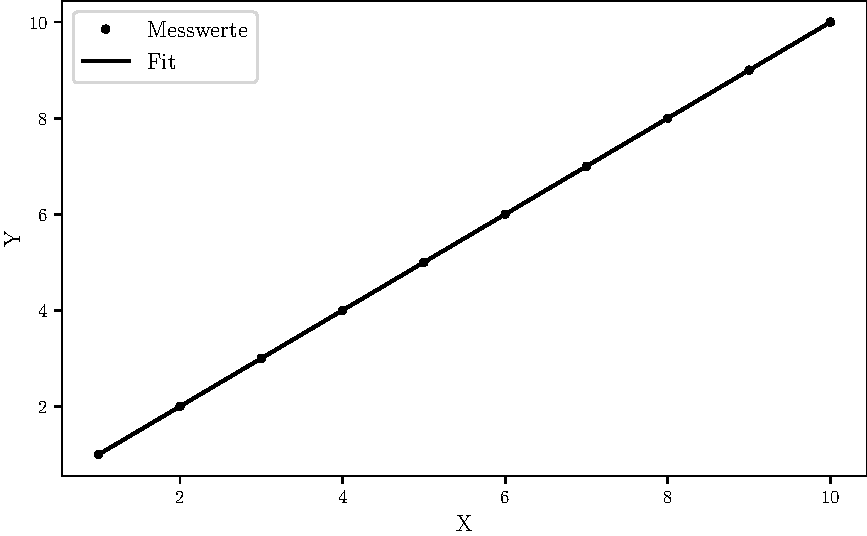
\includegraphics{build/plot.pdf}
%   \caption{Plot}
%   \label{fig:plot}
% \end{figure}
\noindent Die Qualität der Interferenzsignale lässt sich durch den Kontrast $K$
quantifizieren. Um diesen zu ermitteln, wird der initiale Polarisationsfilter
in einem Intervall $\Theta \in [\SI{345}{\degree}, \SI{195}{\degree}]$
in Schritten von je $\theta = \SI{15}{\degree}$ gedreht und die Spannungsextrema
gemessen. Die Messwerte sind in Tabelle \ref{tabular_01} dargelegt. In den
Bereichen um Winkel, an denen der Kontrast besonders auffällig ist, werden
zusätzliche Messungen durchgeführt. 


\section{Diskussion}
Abschließend sollen die berechneten Brechungsindizes mit aktuellen
Literaturwerten verglichen werden, um die Abweichung zu quantisieren. Mögliche
Literaturwerte sind in Tabelle \ref{tabular_05} aufgelistet, wobei die genaue
Zusammensetzung des verwendeten Glases nicht bekannt ist, ebensowenig wie der
Einfluss der Gasdruckröhre selbst (Einlass- und Auslassfenster). \\
\FloatBarrier
\begin{table}
  \centering
  \caption{Aktuelle Litraturwerte für die Brechungsindizes von Glas und Luft.}
  \label{tabular_05}
  \begin{tabular}{c c c c c}
    \toprule
   \multicolumn{1}{c}{Medium} & \multicolumn{1}{c}{$n$} & \multicolumn{1}{c}{Temperatur $T$}
   & \multicolumn{1}{c}{Druck $p$} & \multicolumn{1}{c}{Quellennachweis}\\
   \midrule
    Glas & \num{1.458}  & \SI{20}{\celsius} & \num{1033} & \text{\cite{hecht}} \\
    Luft & \num{1.000293} & \SI{0}{\celsius} & \num{1033} & \text{\cite{hecht}} \\
\bottomrule
  \end{tabular}
\end{table}

\FloatBarrier
\noindent Die berechneten Brechungsindizes wurden Auf Grundlage von Messungen bei
einer gemessenen Temperatur von $T = \SI{20.5}{\celsius}$ gemessen. Für den
berechneten Brechungsindex von Glas $n_\text{Glas} = \num{1.00000128}$ beträgt
die Abweichung etwa $\SI{50}{\percent}$, bei der Messung des Brechungsindexes
von Luft zu beispielsweise $n_\text{Luft} = \num{1.00975}$ beträgt die
Abweichung zum Literaturwert etwa $\SI{1}{\percent}$. Zu beachten ist bei den
Messungen allerdings, dass die angegebenen Literaturwerte bei anderen
Temperaturen bestimmt wurden. Zusätzlich lassen sich Beeinflussungen der
optischen Weglänge durch Druckschwankungen der Luft im Strahlengang des
Interferometers nicht quantifizieren. \\
\noindent Wesentlich für die gemessenen und berechneten Ungenauigkeiten ist
allerdings die Versuchsdurchführung selbst. Wie die Berechnungen des Kontrasts
gezeigt haben, liegt dieser lediglich bei etwa $\SI{88}{\percent}$ des
Idealwertes. Ferner wurde durch die Einlassmethode durch das Öffnen des Ventils
der Druck ungleichmäßig erhöht, was zu Messungenauigkeiten geführt haben kann.


 \newpage
 \nocite{*}
 \printbibliography

\end{document}
